\chapter{The Discovery of the Gluon}

To organize hadrons in dependence on the quantum variables strangeness and isospin Murray Gell-Mann and Yuval Ne'eman proposed independently from each other the Eightfold Way in 1961.
Mesons with a spin parity configuration of $0^-$ and baryons with $\sfrac 12^+$ can both be organized in an octet while baryons with $\sfrac 32^+$ can be organized in a decuplet of which the tenth particle, the $\upOmega^-(sss)$ has been proposed theoretically before it has been found later \cite{Fritzsch2018}.
The early quark model was proposed by Gell-Mann and George Zweig in 1964 which consisted of only $u,\ d,\ s$-quark.
An electron-proton scattering event from 1968 revealed partons that took up half of the carried momentum and were thus the first indication of gluons \cite{Venker}.
A theoretical description is given by Quantum Chromodynamics (QCD) after which the baryon wave function must be antisymmetric thus leading to the introduction of colour as another quantum variable that can be either red, green or blue.
QCD is an $\text{SU}(3)$ gauge symmetry theory that describes the strong interaction predicting eight gluons as gauge bosons that can interact with themselves.
Particles with a colour charge can never be detected as a single particle, because the energy to separate two particles increases until a particle-antiparticle pair is produced, called confinement leading to quarks and gluons combining with other colour-carrying particles forming new hadrons.
These hadrons can in turn form new hadrons themselves building a cascade of particles called a jet which was first observed at the Stanford Positron Electron Asymmetric Rings (SPEAR) at $\SI{7.4}{\giga\eV}$ in 1975.
\begin{wrapfigure}{r}{5.5cm}
    \centering
    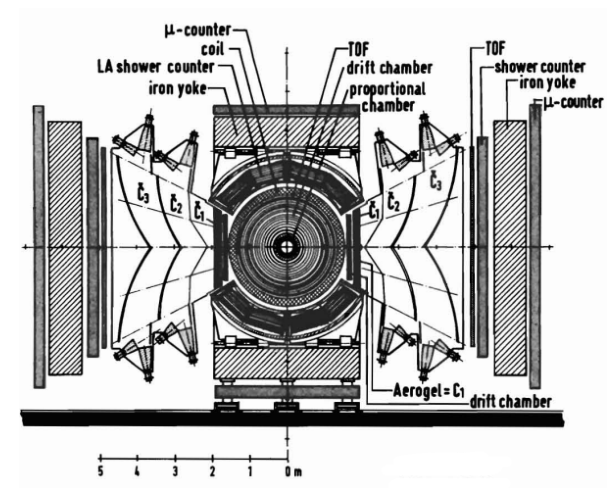
\includegraphics[width=0.4\textwidth]{figs/TASSO.png}
    \caption{Schematic image of the TASSO-detector \cite{TASSO:1979xej}.}
    \label{fig:TASSO}
\end{wrapfigure}
In the year 1979, all quarks except the top quark were found in experiments with the most recent discovery being the bottom quark in 1977 with no experimental evidence for gluons thus far.
Due to corrections at high energies, an electron-positron collision can produce a quark-antiquark pair with an additional gluon in a three-jet event as suggested by John Ellis.
The gluon emission can be seen as the equivalent of bremsstrahlung in QCD.
The transition between a two and a three-jet event is continuous as the jets get broader the higher the energy gets until they can split up into three distinct jets.
A two jet-event starts at energies of $\SI{7.4}{\giga\eV}$ and turns into a three-jet event at $\sim\SI{20}{\giga\eV}$.
The first gluon was discovered in a three-jet event at a center of mass energy of $\SI{27.4}{\giga\eV}$ with the Two Arm Spectrometer Solenoid (TASSO) at the Positron-Electron Tandem Ring Accelerator (PETRA) in 1979 which is part of the Deutsches Elektronen-Synchrotron (DESY).
A schematic picture of TASSO is shown in figure \ref{fig:TASSO}.
It started building in 1976 and was finished just two years later and had a ring accelerator with a circumference of $\SI{2.304}{\kilo\meter}$ that could reach $\SI{27}{\giga\eV}$.
The detector had two hadron-identifying arms, one aerogel and two gas Cherenkov detectors and time-of-flight and shower counters.
Event shape variables were introduced as perturbation theory was not useable for low energies which could be used to distinguish between different QCD models, one in which there are no gluons and one in which there are.
The experimental results were in good agreement with the prediction gluon model, as can be seen in figure \ref{fig:GluonResultsA} that shows predictions for different models \cite{Branson:1994eu}.
By measuring the angle in a Lorentz-boosted center-of-momentum frame, called the Ellis-Karliner angle, it is possible to analyse the spin of the gluon.
The Ellis-Karliner angle distribution from TASSO is shown in figure \ref{fig:GluonResultsB} in which the experimental data matches the theoretical prediction of a vector particle proving that the gluon has a spin of 1 \cite{Venker, Soding:1996zk}.
The discovery of the gluon is the perfect example of theory and experiments working together to discover new parts of physics as the gluon was originally predicted by QCD as a vector boson that could be emitted in three-jet events and was discovered in such an event with the exact characteristics it was predicted to have.

\begin{figure}
    \centering
    \begin{subfigure}[B]{.5\textwidth}   % 1st subfigure
        \centering
        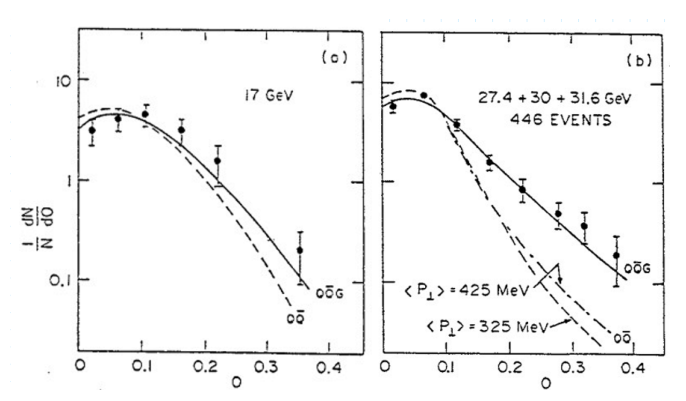
\includegraphics[width=1.1\textwidth]{figs/gluonResultsA.png}
        \caption{Experimental results comparing comparing different QCD models\cite{Branson:1994eu}.}
        \label{fig:GluonResultsA}
    \end{subfigure}
    \begin{subfigure}[B]{.45\textwidth}   % 2nd subfigure
        \centering
        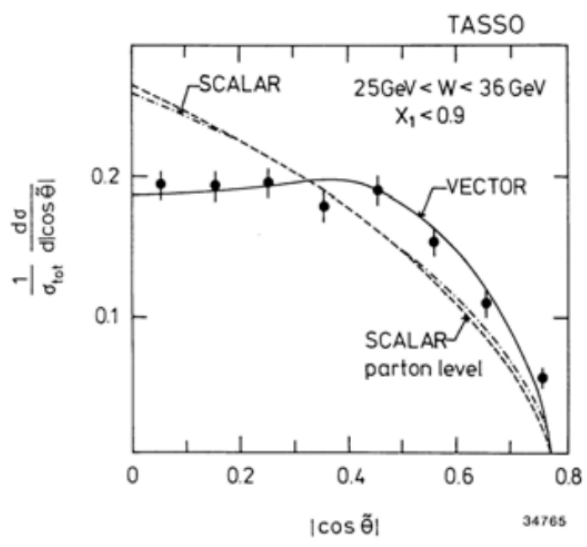
\includegraphics[width=.8\textwidth]{figs/gluonResultsB.png}
        \caption{Ellis-Karliner angle distribution from TASSO \cite{Soding:1996zk}.}
        \label{fig:GluonResultsB}
    \end{subfigure}
    \caption{Experimental results from the TASSO detector \cite{Branson:1994eu, Soding:1996zk}.}
    \label{fig:resultsGluonBoth}
\end{figure}

The strong coupling constant $\alpha_S$ which determines the strength of the interaction can be calculated by measuring the cross-section of three- versus two-jet events.
The compact muon solenoid experiment (CMS) at the large hadron collider (LHC) measured a value of $\alpha_S=\num{0.1448(0.0014)}$ at $\sqrt s=\SI{7}{\tera\eV}$ in 2011 \cite{CMS:2013vbb}.